\mysection{Scenarios}

\mysubsection{Scenario 1}
Giuseppe is an employee of a society. One night, before going to sleep, he receives a call from his chief asking him to attend three meetings in three different zones of Milan. The next day the chief needs to know if Giuseppe can take part in all these meetings or if he has to ask to someone else. Giuseppe has never been in those zones of Milan and, at the moment, he doesn’t have his car because it’s broken. Thus, he has to find another solution.\\
In that moment an idea came in Giuseppe’s mind! He opens the Travlendar+ app on his smartphone and inserted the three events in the calendar, using a TAG called \emph{no car}, which has been specifically created for this situation. This tag includes all the means of transport supported by the app, except the car. During the creation of the last event, Travlendar+ shows to Giuseppe a warning telling him that the event was unreachable on time from the previous one he had set. Knowing this information, Giuseppe calls his chief to inform him that he should ask someone else for the third event only and that he will be able to attend the first two meetings without any problem, because he will use the means suggested by Travlendar+.

\mysubsection{Scenario 2}
Michela is a very busy person and she cares about the environment. She has been very happy to download Travlendar+ on her smartphone, because it can suggest the means of transport that have the less impact on the environment. Thus, every day Michela inserts her events in Travlendar+ and she associates to each one the \emph{CO$_2$ free} preference. In this way, the system gives her the information about all the means of transport available reaching each destination, ordered by the one producing the less CO$_2$ quantity to the one producing the most. This is very useful for Michela, because now she can both follow her wish of having a good impact on the environment and avoid arriving late to her appointments, finding always a good compromise without difficulties.

\mysubsection{Scenario 3}
Luca lives in Milan and on October 20$^{th}$ he has a work meeting in Turin. He decides to insert the meeting in his calendar. As soon as he sets all the data defining the event and concludes the creation, a message appears saying that the event is very far and advices Luca to plan a trip. Luca is very happy of having this opportunity and proceeds on. Travlendar+ provides him an interface in which he can chose between buying a ticket for the train/airplane or adding the ticket if he had already got one. Luca selects the train booking, then Travlendar+ asks Luca to fill up a form containing the date and time he would like to leave, in order to provide him all the solutions with the related starting prices. After a quick look, thanks to the ad-hoc filtration of the trains, Luca is able to choose the most suitable ticket. As soon as he decides to purchase it, two things happen: 
\begin{itemize}
	\setlength{\leftskip}{0.5cm}
	\item a travel event with all the information is automatically created;
	\item Luca is addressed to the travel service website to complete the purchase.
\end{itemize}
Luca will be able to check the solutions to reach the station on time in any moment tapping on the travel event.
When Luca returns on the application, he inserts the period of staying and his accommodation in Turin. So Travlendar+ advices him to buy the local tickets representing the best compromise between price and utility.

\mysubsection{Scenario 4}
Sean lives in Milan and he has to attend a work-lunch in Rome tomorrow. He already has the ticket to reach Rome, because his company took care of it. Thus, he wants to add the travel event in Travlendar+. Nothing simpler! Sean has only to tap for about one second on the screen and the calendar interface will provide him two choices: \emph{create an event} and \emph{plan a trip}. Tapping on plan a trip, Travlendar+ will show an interface where he can insert the info related to the ticket his company provided him and finally create the related travel event.

\mysubsection{Scenario 5}
Gianluca is a financial expert, he has always to attend many meetings during the day and sometimes he forgets to take a break. He needs something to remind him to reserve some time for having lunch. Travlendar+ is the perfect solution to his needs. Gianluca sets in the preferences the time window in which he would like to have lunch, between 12 and 14, and the preferred duration, 60 minutes.\\
Today Gianluca has to add to his calendar one event from 12:00 to 13:00 and another one from 13:30 to 15:00. Travlendar+, given the Gianluca’s setting for the lunch, has already automatically created an event lunch every day from 12:00 to 13.00. When Gianluca adds the first event, the lunch break slides automatically and covers the period between 13.00 and 14.00 without giving any problems. When he tries to insert the second event, a problem come up! In fact, Gianluca will not be able to have a lunch of 60 minutes. Despite this, Travlendar+ must reserve at least 30 minutes for everyday lunch to each user, so it asks Gianluca if he wants to reduce his lunchtime to 30 minutes or postpone the event. Gianluca cannot postpone the event, so he decides to reduce his lunch duration to 30 minutes for tomorrow, leaving the other lunch events unchanged.

\newpage
\mysubsection{Scenario 6}
Gabriele had inserted in his Travlendar+ application his girlfriend tonight’s party event. He had completely forgotten about it, but fortunately, Travlendar+ is sending him warnings to remind him to go to the event whenever the time for reaching the party’s location, without arriving late, with the slowest mean of transport in the list is going to expire. However, during almost all these warnings Gabriele was sleeping and he did not read them. He just gets the last one, which advices him to use the car. Unfortunately, Gabriele doesn’t have a car in Milan but he has the driving licence and he can take a car sharing. Travlendar+ is perfect for Gabriele’s situation! In fact, when he taps on the car choice, the app opens an interface that asks Gabriele to choose between his own car and a car sharing. Choosing the second one, Gabriele is able to see the route for reaching the nearest car location and he is also addressed to the car sharing service app in order to book and reach his girlfriend party’s location on time. Travlendar+ is also able to show him the fastest route to reach his destination.

\newpage
\mysection{Sequence Diagrams}
\mysubsection{Event Creation}
\begin{figure}[H]
	\centering
	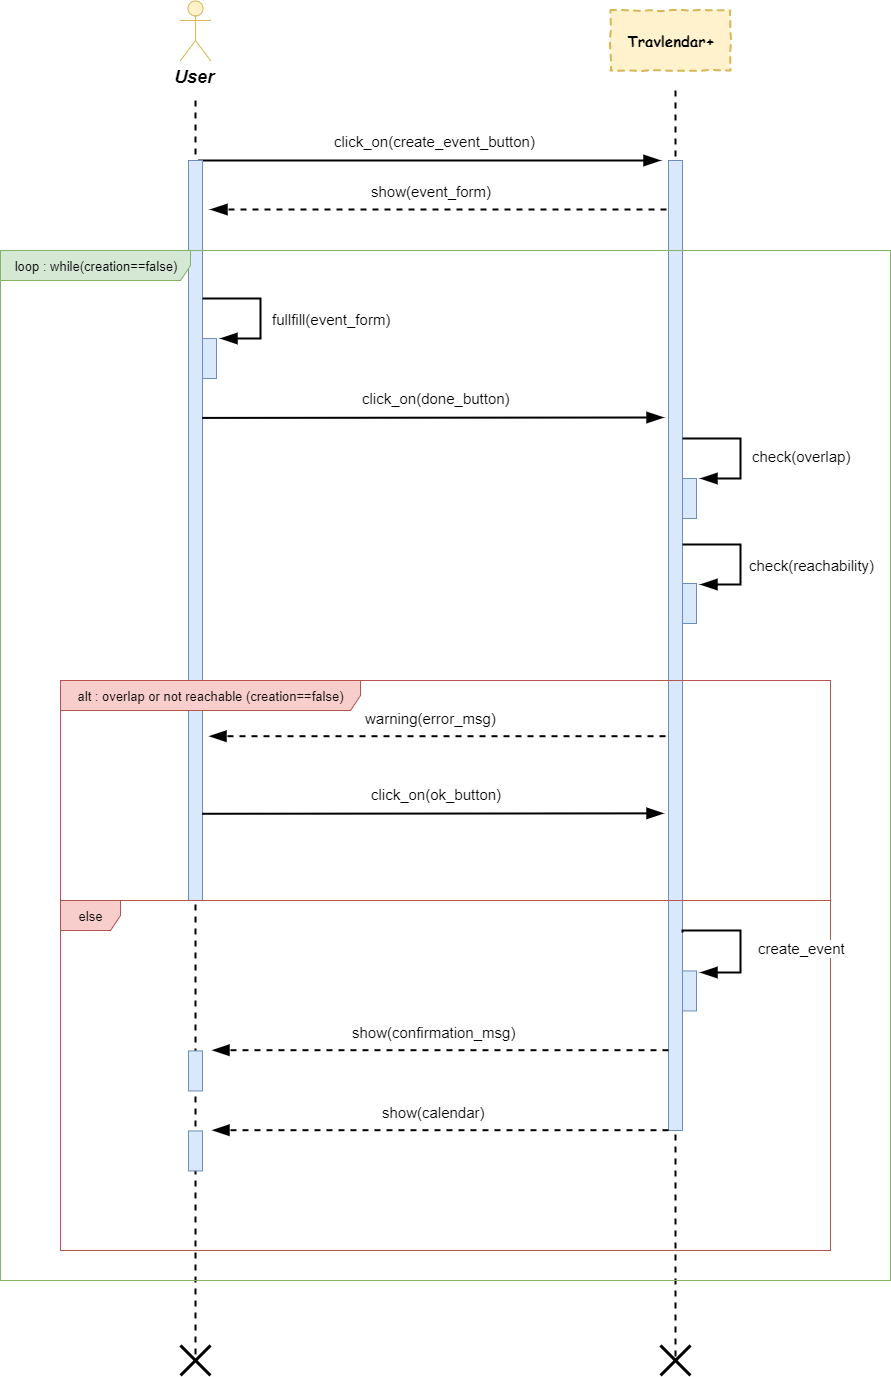
\includegraphics[scale=0.3]{Images/Sequence/Event_Creation}
	\caption{Event Creation Sequence Diagram}
\end{figure}

\mysubsection{Trip Transport Ticket Purchasing}
\begin{figure}[H]
	\centering
	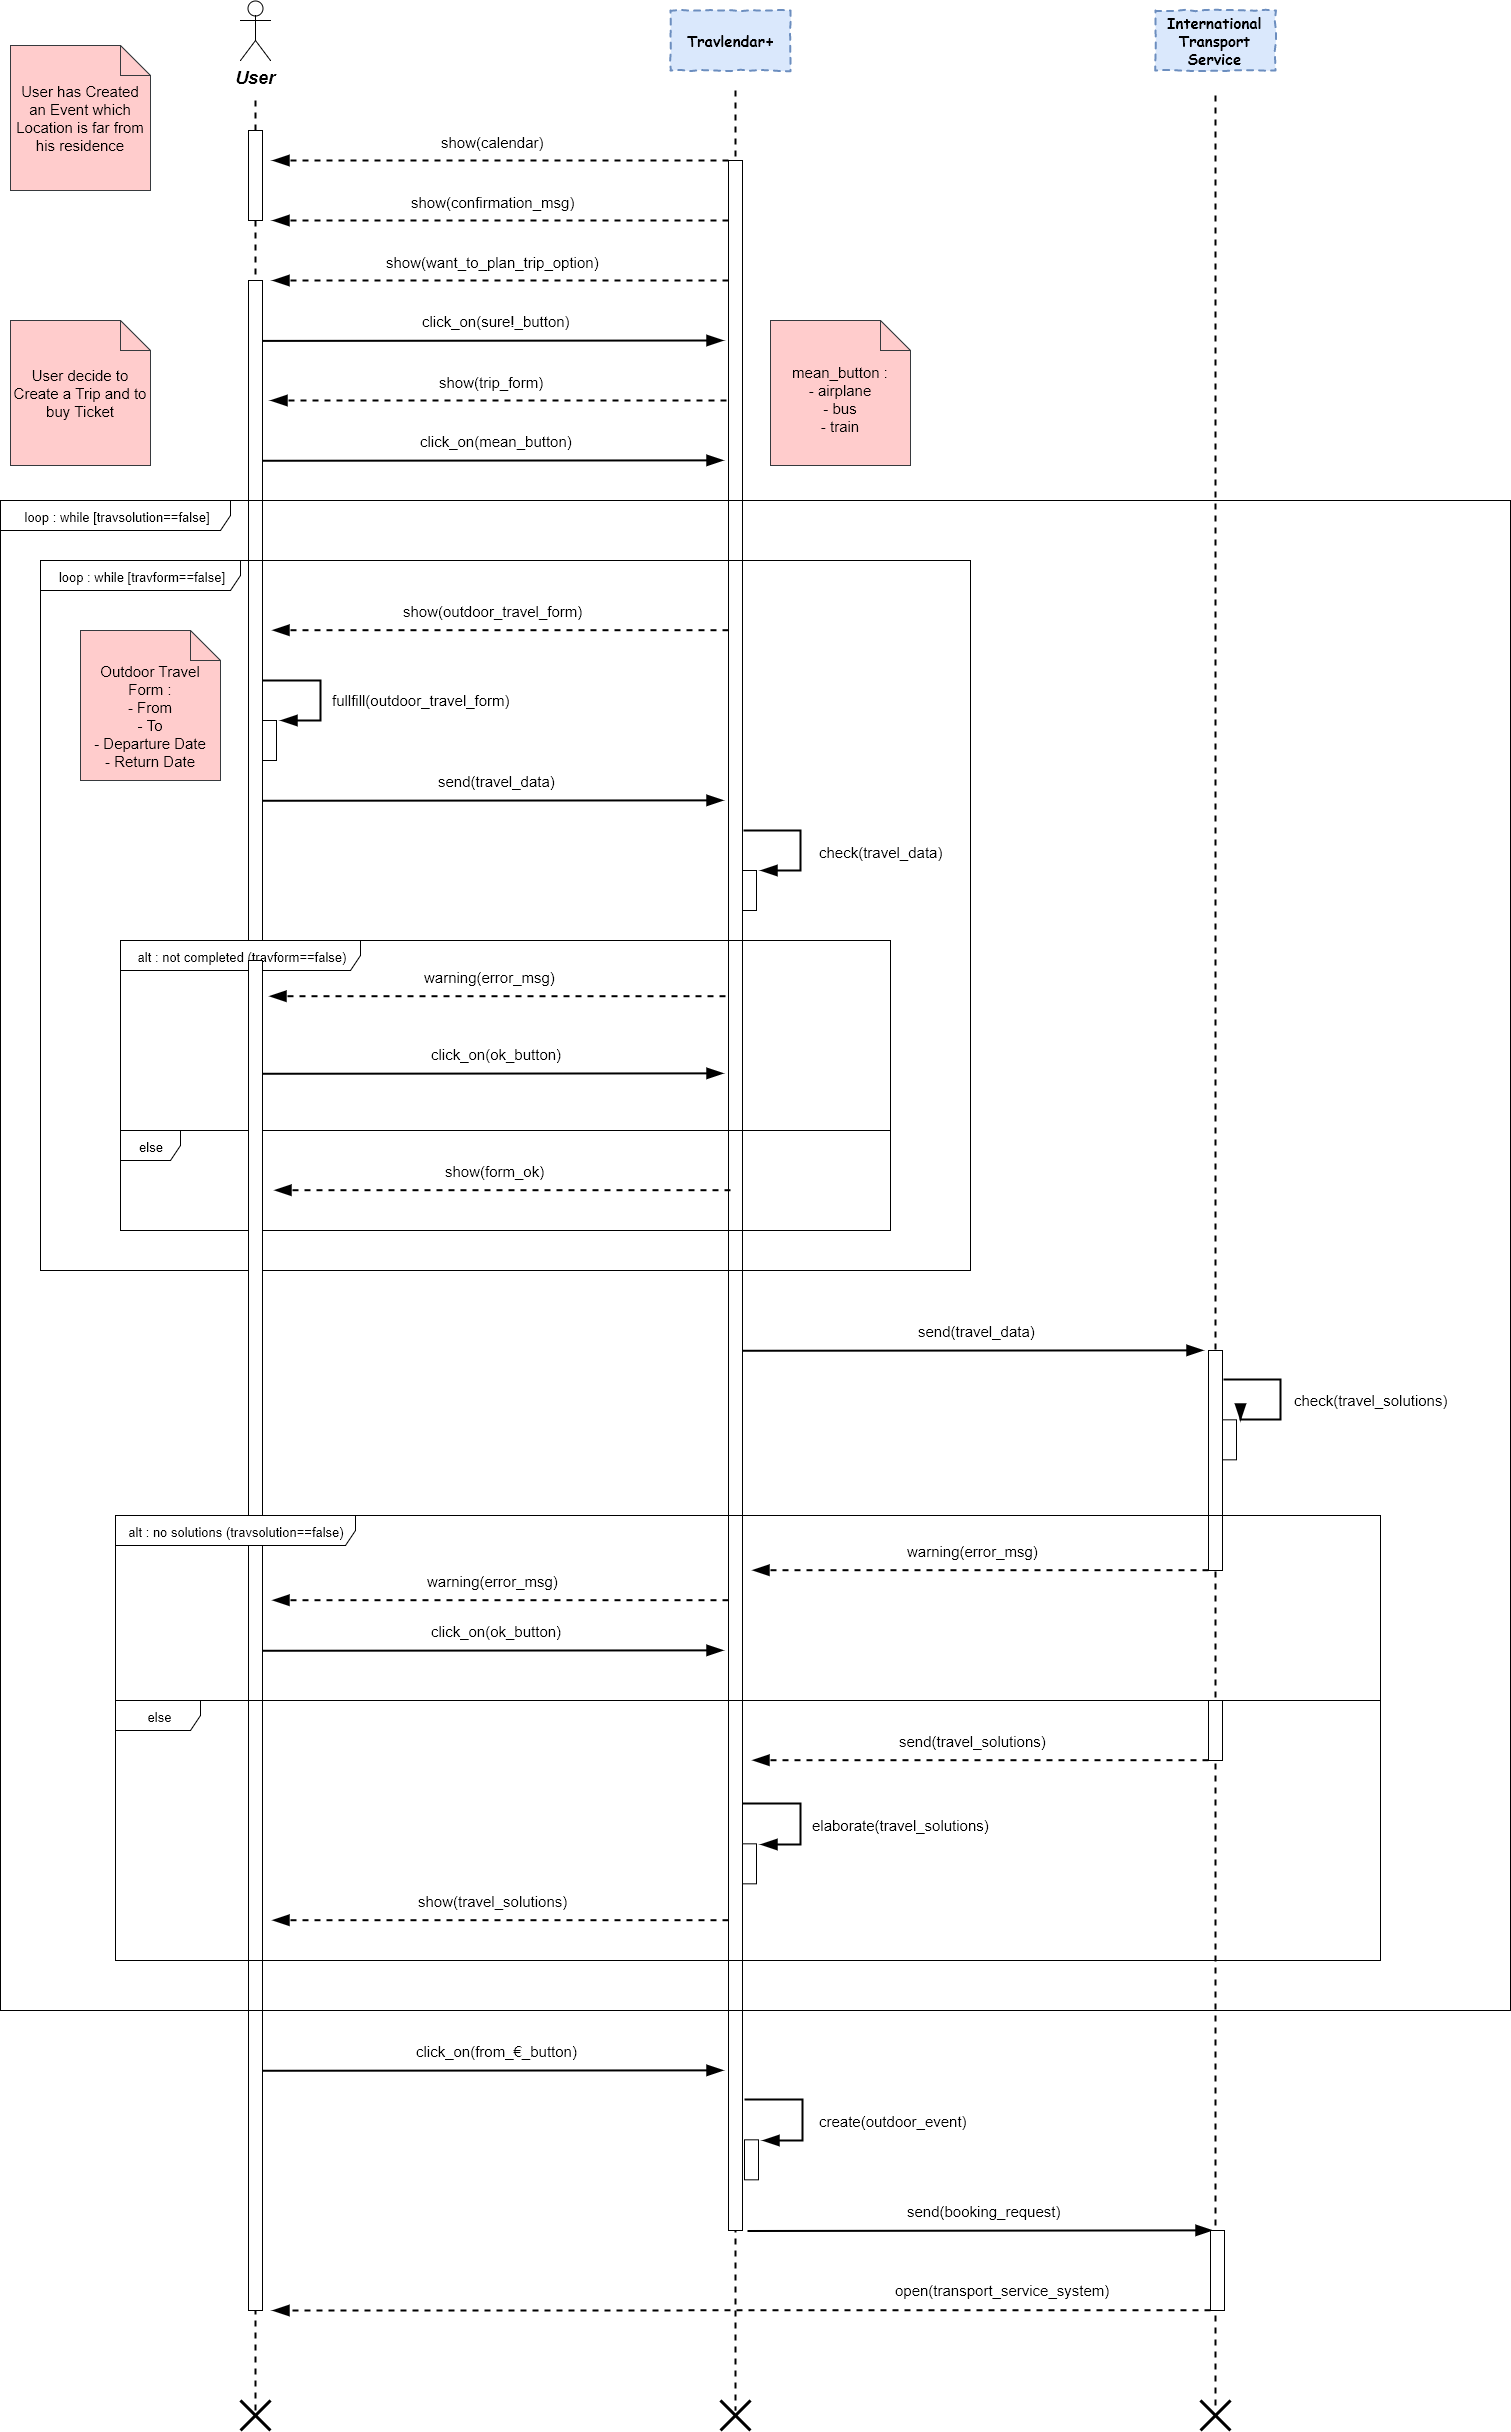
\includegraphics[scale=0.23]{Images/Sequence/Trip_Transport_Ticket_Purchasing}
	\caption{Trip Transport Ticket Purchasing Sequence Diagram}
\end{figure}

\mysubsection{Local Transport Ticket Purchasing}
\begin{figure}[H]
	\centering
	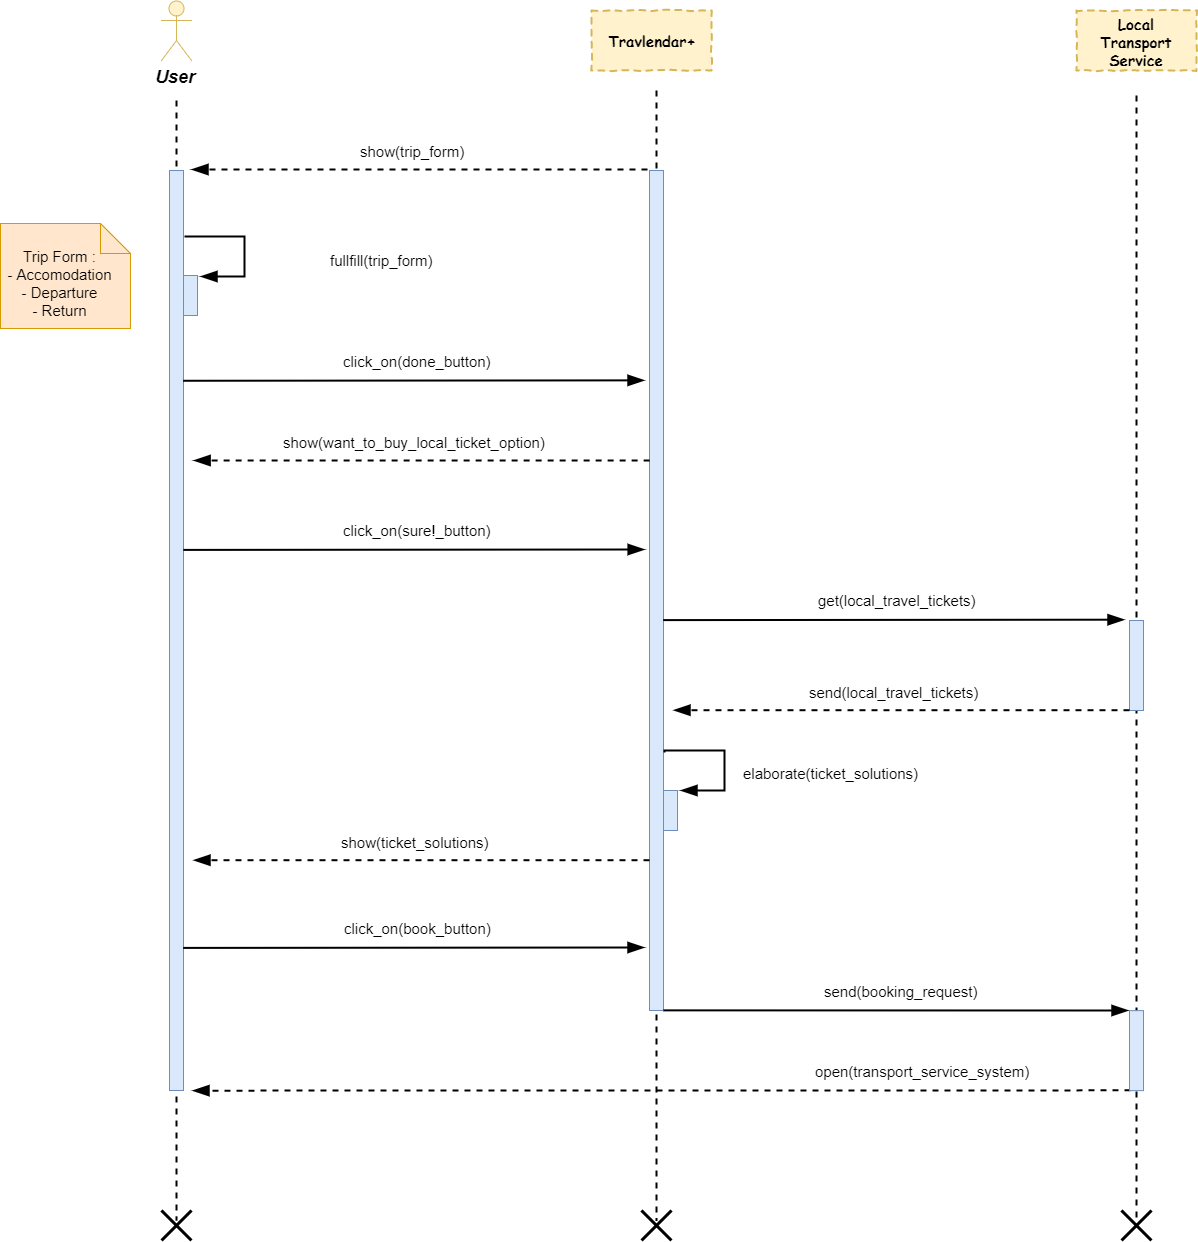
\includegraphics[scale=0.3]{Images/Sequence/Local_Transport_Ticket_Purchasing}
	\caption{Local Transport Ticket Purchasing Sequence Diagram}
\end{figure}

\newpage
\mysection{Activity Diagrams}
\mysubsection{Event Route Computation}
\begin{figure}[H]
	\centering
	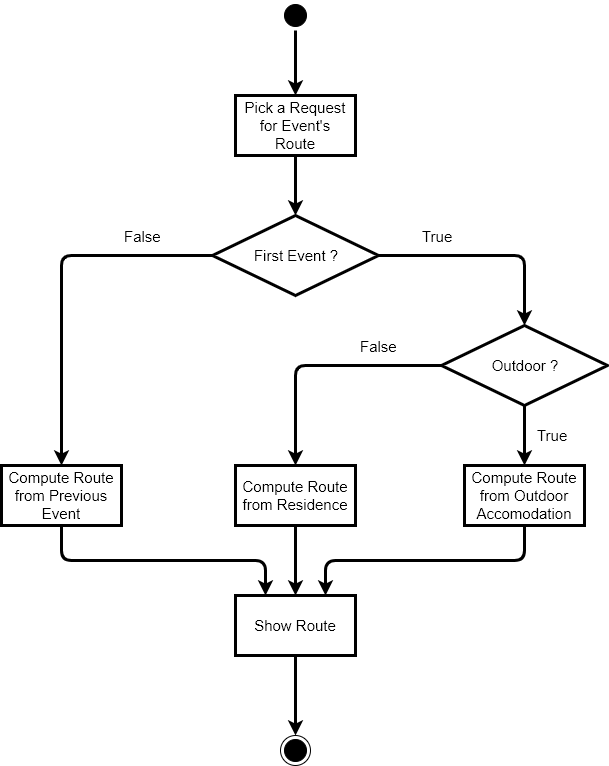
\includegraphics[scale=0.4]{Images/Activity/Event_Route_Computation}
	\caption{Event Route Computation Activity Diagram}
\end{figure}

\mysubsection{Trip Creation}
\begin{figure}[H]
	\centering
	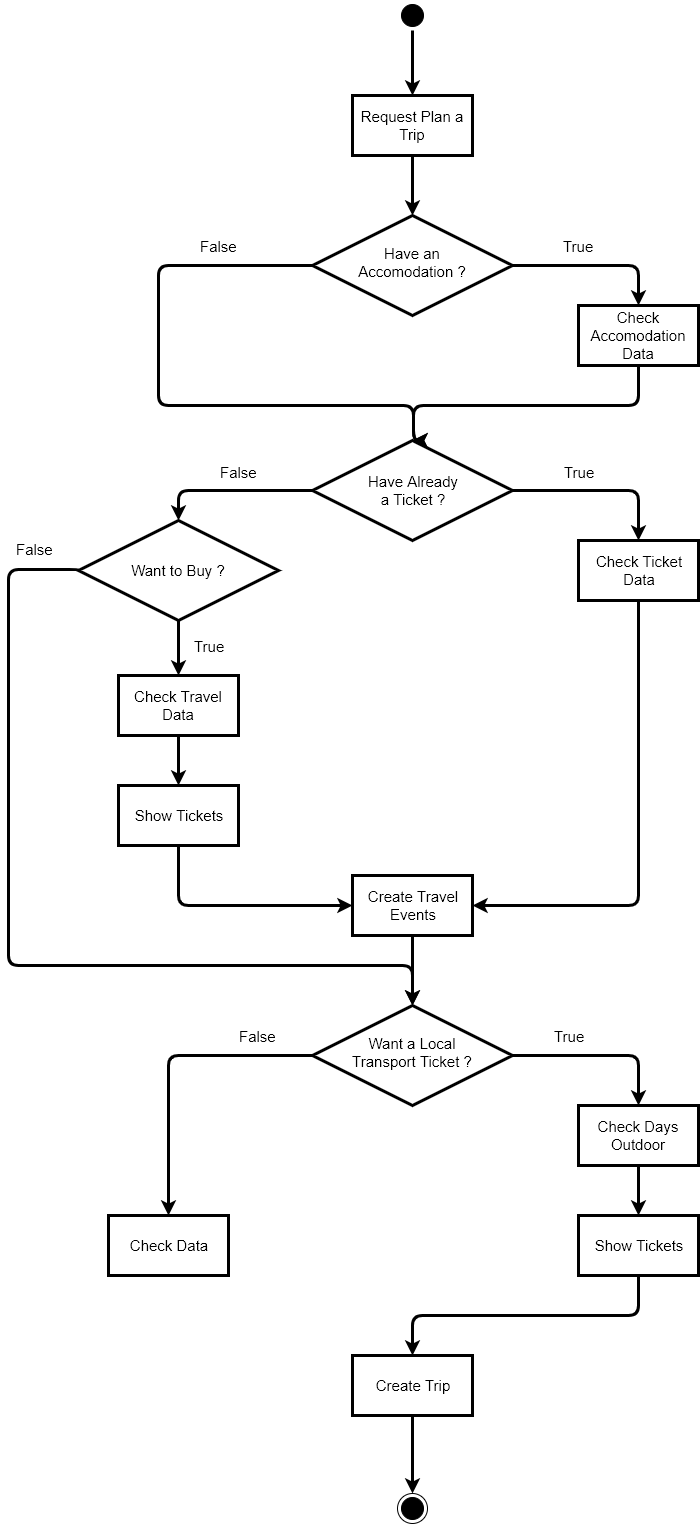
\includegraphics[scale=0.35]{Images/Activity/Trip_Creation}
	\caption{Trip Creation Activity Diagram}
\end{figure}